\documentclass{ximera}
\graphicspath{  %% When looking for images,
{./}            %% look here first,
{./pictures/}   %% then look for a pictures folder,
{../pictures/}  %% which may be a directory up.
{../../pictures/}  %% which may be a directory up.
{../../../pictures/}  %% which may be a directory up.
{../../../../pictures/}  %% which may be a directory up.
}

\usepackage{listings}
%\usepackage{circuitikz}
\usepackage{xcolor}
\usepackage{amsmath,amsthm}
\usepackage{subcaption}
\usepackage{graphicx}
\usepackage{tikz}
%\usepackage{tikz-3dplot}
\usepackage{amsfonts}
%\usepackage{mdframed} % For framing content
%\usepackage{tikz-cd}

  \renewcommand{\vector}[1]{\left\langle #1\right\rangle}
  \newcommand{\arrowvec}[1]{{\overset{\rightharpoonup}{#1}}}
  \newcommand{\ro}{\texttt{R}}%% row operation
  \newcommand{\dotp}{\bullet}%% dot product
  \renewcommand{\l}{\ell}
  \let\defaultAnswerFormat\answerFormatBoxed
  \usetikzlibrary{calc,bending}
  \tikzset{>=stealth}
  




%make a maroon color
\definecolor{maroon}{RGB}{128,0,0}
%make a dark blue color
\definecolor{darkblue}{RGB}{0,0,139}
%define the color fourier0 to be the maroon color
\definecolor{fourier0}{RGB}{128,0,0}
%define the color fourier1 to be the dark blue color
\definecolor{fourier1}{RGB}{0,0,139}
%define the color fourier 1t to be the light blue color
\definecolor{fourier1t}{RGB}{173,216,230}
%define the color fourier2 to be the dark green color
\definecolor{fourier2}{RGB}{0,100,0}
%define teh color fourier2t to be the light green color
\definecolor{fourier2t}{RGB}{144,238,144}
%define the color fourier3 to be the dark purple color
\definecolor{fourier3}{RGB}{128,0,128}
%define the color fourier3t to be the light purple color
\definecolor{fourier3t}{RGB}{221,160,221}
%define the color fourier0t to be the red color
\definecolor{fourier0t}{RGB}{255,0,0}
%define the color fourier4 to be the orange color
\definecolor{fourier4}{RGB}{255,165,0}
%define the color fourier4t to be the darker orange color
\definecolor{fourier4t}{RGB}{255,215,0}
%define the color fourier5 to be the yellow color
\definecolor{fourier5}{RGB}{255,255,0}
%define the color fourier5t to be the darker yellow color
\definecolor{fourier5t}{RGB}{255,255,100}
%define the color fourier6 to be the green color
\definecolor{fourier6}{RGB}{0,128,0}
%define the color fourier6t to be the darker green color
\definecolor{fourier6t}{RGB}{0,255,0}

%New commands for this doc for errors in copying
\newcommand{\eigenvar}{\lambda}
%\newcommand{\vect}[1]{\mathbf{#1}}
\renewcommand{\th}{^{\text{th}}}
\newcommand{\st}{^{\text{st}}}
\newcommand{\nd}{^{\text{nd}}}
\newcommand{\rd}{^{\text{rd}}}
\newcommand{\paren}[1]{\left(#1\right)}
\newcommand{\abs}[1]{\left|#1\right|}
\newcommand{\R}{\mathbb{R}}
\newcommand{\C}{\mathbb{C}}
\newcommand{\Hilb}{\mathbb{H}}
\newcommand{\qq}[1]{\text{#1}}
\newcommand{\Z}{\mathbb{Z}}
\newcommand{\N}{\mathbb{N}}
\newcommand{\q}[1]{\text{``#1''}}
%\newcommand{\mat}[1]{\begin{bmatrix}#1\end{bmatrix}}
\newcommand{\rref}{\text{reduced row echelon form}}
\newcommand{\ef}{\text{echelon form}}
\newcommand{\ohm}{\Omega}
\newcommand{\volt}{\text{V}}
\newcommand{\amp}{\text{A}}
\newcommand{\Seq}{\textbf{Seq}}
\newcommand{\Poly}{\textbf{P}}
\renewcommand{\quad}{\text{    }}
\newcommand{\roweq}{\simeq}
\newcommand{\rowop}{\simeq}
\newcommand{\rowswap}{\leftrightarrow}
\newcommand{\Mat}{\textbf{M}}
\newcommand{\Func}{\textbf{Func}}
\newcommand{\Hw}{\textbf{Hamming weight}}
\newcommand{\Hd}{\textbf{Hamming distance}}
\newcommand{\rank}{\text{rank}}
\newcommand{\longvect}[1]{\overrightarrow{#1}}
% Define the circled command
\newcommand{\circled}[1]{%
  \tikz[baseline=(char.base)]{
    \node[shape=circle,draw,inner sep=2pt,red,fill=red!20,text=black] (char) {#1};}%
}

% Define custom command \strikeh that just puts red text on the 2nd argument
\newcommand{\strikeh}[2]{\textcolor{red}{#2}}

% Define custom command \strikev that just puts red text on the 2nd argument
\newcommand{\strikev}[2]{\textcolor{red}{#2}}

%more new commands for this doc for errors in copying
\newcommand{\SI}{\text{SI}}
\newcommand{\kg}{\text{kg}}
\newcommand{\m}{\text{m}}
\newcommand{\s}{\text{s}}
\newcommand{\norm}[1]{\left\|#1\right\|}
\newcommand{\col}{\text{col}}
\newcommand{\sspan}{\text{span}}
\newcommand{\proj}{\text{proj}}
\newcommand{\set}[1]{\left\{#1\right\}}
\newcommand{\degC}{^\circ\text{C}}
\newcommand{\centroid}[1]{\overline{#1}}
\newcommand{\dotprod}{\boldsymbol{\cdot}}
%\newcommand{\coord}[1]{\begin{bmatrix}#1\end{bmatrix}}
\newcommand{\iprod}[1]{\langle #1 \rangle}
\newcommand{\adjoint}{^{*}}
\newcommand{\conjugate}[1]{\overline{#1}}
\newcommand{\eigenvarA}{\lambda}
\newcommand{\eigenvarB}{\mu}
\newcommand{\orth}{\perp}
\newcommand{\bigbracket}[1]{\left[#1\right]}
\newcommand{\textiff}{\text{ if and only if }}
\newcommand{\adj}{\text{adj}}
\newcommand{\ijth}{\emph{ij}^\text{th}}
\newcommand{\minor}[2]{M_{#2}}
\newcommand{\cofactor}{\text{C}}
\newcommand{\shift}{\textbf{shift}}
\newcommand{\startmat}[1]{
  \left[\begin{array}{#1}
}
\newcommand{\stopmat}{\end{array}\right]}
%a command to give a name to explorations and hints and theorems
\newcommand{\name}[1]{\begin{centering}\textbf{#1}\end{centering}}
\newcommand{\vect}[1]{\vec{#1}}
\newcommand{\dfn}[1]{\textbf{#1}}
\newcommand{\transpose}{\mathsf{T}}
\newcommand{\mtlb}[2][black]{\texttt{\textcolor{#1}{#2}}}
\newcommand{\RR}{\mathbb{R}} % Real numbers
\newcommand{\id}{\text{id}}
\newcommand{\coord}[1]{\langle#1\rangle}
\newcommand{\RREF}{\text{RREF}}
\newcommand{\Null}{\text{Null}}
\newcommand{\Nullity}{\text{Nullity}}
\newcommand{\Rank}{\text{Rank}}
\newcommand{\Col}{\text{Col}}
\newcommand{\Ef}{\text{EF}}
\newcommand{\boxprod}[3]{\abs{(#1\times#2)\cdot#3}}

\author{Zack Reed}
%borrowed from selinger linear algebra
\title{Planes Revisited}
\begin{document}
\begin{abstract}

    In this learning activity, you will be 
\end{abstract}
\maketitle

\section*{Planes in $\RR^3$}
 
You are probably familiar with the expression ``two points determine a line."  This means that given two distinct points, there is exactly one line that passes through both of them.  There are other ways to describe a line.  For example, as we saw in \href{https://ximera.osu.edu/oerlinalg/LinearAlgebra/RRN-0020/main}{Parametric Equations of Lines}, a single point together with a direction vector also determine a line.
 
You are probably also familiar with the fact that three non-collinear points determine a plane. (This is why photographers use tripods for stability, while four-legged chairs often wobble!)  Is there another way to determine a plane? 
 
The diagram below shows several planes perpendicular to vector $\vec{n}$.  In fact, there are infinitely many such planes.  Vector $\vec{n}$ does not determine a plane, but if we know of a point $P$ contained in the plane, then together, $P$ and $\vec{n}$ describe a unique plane.
 
 \begin{center}
\tdplotsetmaincoords{70}{130}
    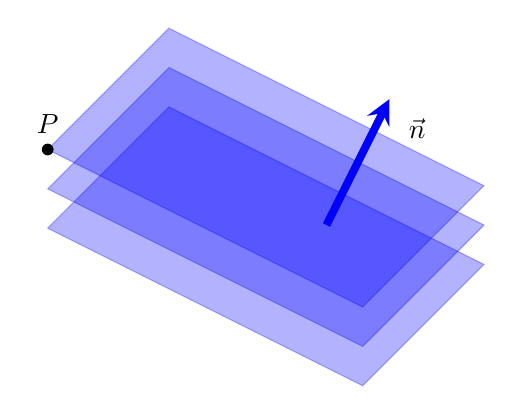
\begin{tikzpicture}[scale=1]
 
\filldraw[blue, opacity=0.3] (2,-1,2)--(2,-1,-2)--(-2,1,-2)--(-2,1,2)--cycle;
 
\filldraw[blue, opacity=0.3] (2,-0.5,2)--(2,-0.5,-2)--(-2,1.5,-2)--(-2,1.5,2)--cycle;
 
\filldraw[blue, opacity=0.3] (2,-1.5,2)--(2,-1.5,-2)--(-2,0.5,-2)--(-2,0.5,2)--cycle;
 
    \draw[line width=1mm, -stealth, blue](0,-1,-2)--(0.8,0.6,-2) ;%normal to grey
    \node[fill,circle,inner sep=1.5pt,label={$P$}] at (-2,1.5,2) {};
    \node[label={below right:$\vec{n}$}] at (0.8,0.6,-2) {};
     \end{tikzpicture}
           
     \end{center}

 
\begin{definition}[Normal Vector]\label{def:normalvectoplane}
A nonzero vector $\vec{n}$ is called a \dfn{normal} for a plane if it is orthogonal to every vector in the plane.
\end{definition}
 
\begin{example}\label{ex:standardunitvectnormals}
The standard unit vector $\vec{k}$ is orthogonal to every vector in the $xy$-plane, therefore it is a normal for the $xy$-plane.
 
\begin{center}
\tdplotsetmaincoords{70}{130}
    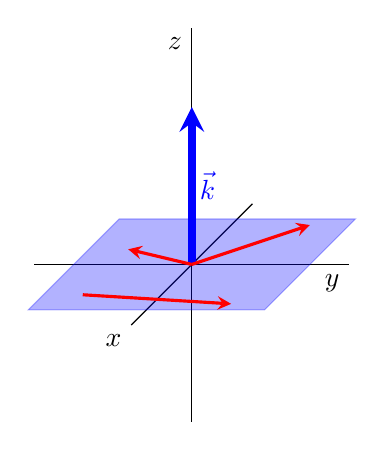
\begin{tikzpicture}[scale=1]
 
\draw(-2,0,0)--(2,0,0) node[below left]{$y$};
    \draw(0,-2,0)--(0,3,0) node[below left]{$z$};
    \draw(0,0,-2)--(0,0,2) node[below left]{$x$};
\filldraw[blue, opacity=0.3] (1.5,0,1.5)--(-1.5,0,1.5)--(-1.5,0,-1.5)--(1.5,0,-1.5)--cycle;
     
    \draw[blue,line width=1mm, -stealth](0,0,0)--(0,2,0) ;
     
    \node[blue] at (0.2, 1, 0)   {$\vec{k}$};
 
\draw[line width=0.4mm, -stealth, red](0,0,0)--(1,0,-1.3) ;
 
\draw[line width=0.4mm, -stealth, red](-1,0,1)--(1,0,1.3) ;
 
\draw[line width=0.4mm, -stealth, red](0,0,0)--(-1,0,-0.5) ;
 
\end{tikzpicture}
\end{center}
\end{example}

 
Given a point $P_{0} = P_{0}(x_{0}, y_{0}, z_{0})$ and a nonzero vector $\vec{n}$, there is a unique plane through $P_{0}$ with normal $\vec{n}$.
 
\begin{center}
\tdplotsetmaincoords{70}{130}
    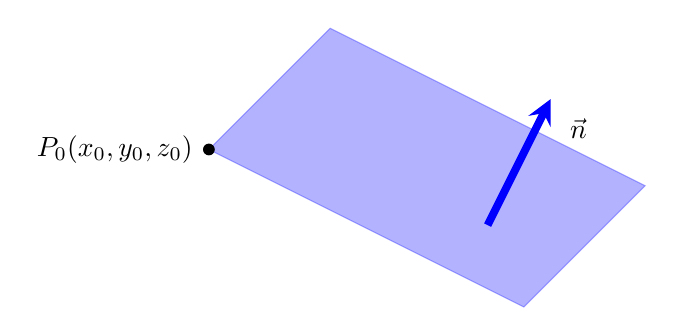
\begin{tikzpicture}[scale=1]
 
\filldraw[blue, opacity=0.3] (2,-0.5,2)--(2,-0.5,-2)--(-2,1.5,-2)--(-2,1.5,2)--cycle;
 
    \draw[line width=1mm, -stealth, blue](0,-1,-2)--(0.8,0.6,-2) ;%normal to grey
    \node[fill,circle,inner sep=1.5pt,label={left:$P_0(x_0, y_0, z_0)$}] at (-2,1.5,2) {};
    \node[label={below right:$\vec{n}$}] at (0.8,0.6,-2) {};
    \end{tikzpicture}
           
\end{center}


 
This fact can be used to give a very simple description of a
plane.
 Observe that a point $P = P(x, y, z)$ lies on this plane if and only if the vector $\overrightarrow{P_{0}P}$ is orthogonal to $\vec{n}$ (i.e. $P$ lies in the plane if and only if $\vec{n} \dotp \overrightarrow{P_{0}P} = 0$).
  
 \begin{center}
\tdplotsetmaincoords{70}{130}
    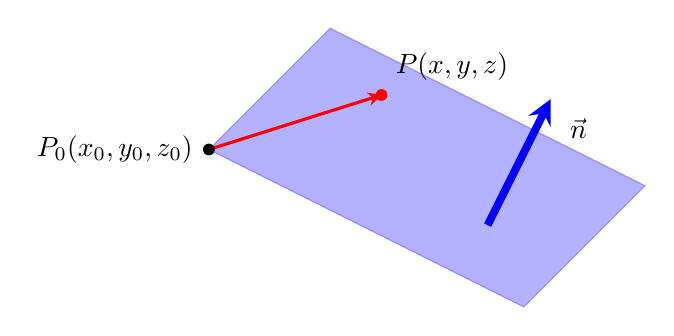
\begin{tikzpicture}[scale=1]
 
\filldraw[blue, opacity=0.3] (2,-0.5,2)--(2,-0.5,-2)--(-2,1.5,-2)--(-2,1.5,2)--cycle;
 
    \draw[line width=1mm, -stealth, blue](0,-1,-2)--(0.8,0.6,-2) ;%normal to grey
     
    \node[fill,red,circle,inner sep=1.5pt,label={above right:$P(x, y, z)$}] at (0,2,1.5) {};
    \node[label={below right:$\vec{n}$}] at (0.8,0.6,-2) {};
     
    \draw[line width=0.4mm, -stealth, red](-2,1.5,2)--(0,2,1.5) ;
     
    \node[fill,circle,inner sep=1.5pt,label={left:$P_0(x_0, y_0, z_0)$}] at (-2,1.5,2) {};
    \end{tikzpicture}
           
\end{center}


  
Let $\vec{n}=\begin{bmatrix}a\\b\\c\end{bmatrix}$.  By ``head-tail" formula, we have: $\overrightarrow{P_{0}P} = \begin{bmatrix}
x - x_{0}\\
y - y_{0}\\
z - z_{0}
\end{bmatrix}$. So, $P(x, y, z)$ lies in the plane if and only if
$$\begin{bmatrix}a\\b\\c\end{bmatrix}\dotp\begin{bmatrix}
x - x_{0}\\
y - y_{0}\\
z - z_{0}
\end{bmatrix}=a(x-x_0)+b(y-y_0)+c(z-z_0)=0$$
We summarize this result as a theorem.
 
\begin{theorem}\label{th:scalareqofplane}
The plane through $P_{0}(x_{0}, y_{0}, z_{0})$ with a normal vector $$\vec{n} =
\begin{bmatrix}
a\\
b\\
c
\end{bmatrix}\neq\vec{0}$$
 is given by
\begin{equation}\label{eq:plane}
a(x - x_{0}) + b(y - y_{0}) + c(z - z_{0}) = 0
\end{equation}
\end{theorem}
 
\begin{example}\label{ex:planewithnormalvector}
Find an equation of the plane through $P_{0}(1, -1, 3)$ with $\vec{n} =
\begin{bmatrix}
3\\
-1\\
2
\end{bmatrix}$
 as a normal vector.
\begin{explanation}
  Here the equation becomes
\begin{equation*}
3(x - 1) - (y + 1) + 2(z - 3) = 0
\end{equation*}
This simplifies to $3x - y + 2z = 10$.
 
GeoGebra interactive below shows the plane, together with point $P_0$ and the normal vector.  RIGHT-CLICK and DRAG to rotate the image for a better view.

          

 
\pdfOnly{
Access GeoGebra interactives through the online version of this text at
 
\href{https://ximera.osu.edu/oerlinalg}{https://ximera.osu.edu/oerlinalg}.
}
 
\begin{onlineOnly}
\begin{center}
\geogebra{gsaag2dx}{900}{600}
\end{center}
\end{onlineOnly}
 
\end{explanation}
\end{example}

 
As demonstrated in Example \ref{ex:planewithnormalvector}, we can distribute coefficients $a$, $b$ and $c$  of equation (\ref{eq:plane}) as follows:
$$ax-ax_0+by-by_0+cz-cz_0=0$$
Setting $d = ax_{0} + by_{0} + cz_{0}$, shows that every plane with a normal vector $\vec{n} =
\begin{bmatrix}
a\\
b\\
c
\end{bmatrix}$
 has a linear equation of the form
\begin{equation} \label{eq:eqofline}
ax + by + cz = d
\end{equation}
for some constant $d$. Conversely, the graph of this equation is a plane with $\vec{n} =
\begin{bmatrix}
a\\
b\\
c
\end{bmatrix}$ as a normal vector (assuming that $a$, $b$, and $c$ are not all zero).
 
 
\begin{example}\label{ex:planeparalleltoplane}
Find an equation of the plane through $P_{0}(3, -1, 2)$ that is parallel to the plane with equation $2x - 3y = 6$.
 
\begin{explanation}
The plane with equation $2x -3y = 6$ has a normal vector $\vec{n} =
\begin{bmatrix}
2\\
-3\\
0
\end{bmatrix}$. Because the two planes are parallel, $\vec{n}$ serves as a normal for the plane we seek, so the equation is $2x - 3y = d$ for some $d$ by (\ref{eq:eqofline}). Insisting that $P_{0}(3, -1, 2)$ lies on the plane determines $d$; that is, $d = 2 \cdot 3 - 3(-1) = 9$. Hence, the equation is $2x - 3y = 9$.
 
GeoGebra interactive below shows the two planes, together with point $P_0$ and the normal vector.  RIGHT-CLICK and DRAG to rotate the image for a better view.
 
\pdfOnly{
Access GeoGebra interactives through the online version of this text at
 
\href{https://ximera.osu.edu/oerlinalg}{https://ximera.osu.edu/oerlinalg}.
}
 
\begin{onlineOnly}
\begin{center}
\geogebra{unceva9g}{900}{600}
\end{center}
\end{onlineOnly}
\end{explanation}
\end{example}


 
\subsection*{Linear Equations and their Graphs: From Lines to Hyperplanes}
An equation of the form $ax+by=d$ is a linear equation whose graph is a line in $\RR^2$. If we solve for $y$ in terms of $x$, we obtain a more familiar form of this equation, $y=-\frac{a}{b}x+\frac{d}{b}$.  The slope of the corresponding line is $m=-\frac{a}{b}$.  Observe that a line perpendicular to this line has the slope $\frac{b}{a}$.  If we interpret $a$ as a horizontal ``run" and $b$ as a vertical ``rise", we see that the vector $\begin{bmatrix}a\\b\end{bmatrix}$ is perpendicular to the line $ax+by=d$.  You can use the following GeoGebra interactive to solidify your understanding of this.


 
\pdfOnly{
Access GeoGebra interactives through the online version of this text at
 
\href{https://ximera.osu.edu/oerlinalg}{https://ximera.osu.edu/oerlinalg}.
}
 
\begin{onlineOnly}
\begin{center}
\geogebra{tg2duwqk}{900}{600}
\end{center}
\end{onlineOnly}
 
The idea of coefficients in front of variables forming components of a normal vector should be very familiar to you.  Recall that the graph of $ax+by+cz=d$ is a plane in $\RR^3$ with a normal vector $\vec{n}=\begin{bmatrix}a\\b\\c\end{bmatrix}$.


 
Lines and planes may seem very different, but they are all graphs of linear equations, just in different dimensions.  In general, an equation of the form
$$a_1x_1+a_2x_2+\dots +a_nx_n=d$$
is called a \dfn{linear equation} in $n$ variables.  The graph of such an equation, for $3$, is called a \dfn{hyperplane}.  The vector in $\RR^n$ whose components are the coefficients $a_1, a_2, \dots ,a_n$ is orthogonal to every vector in the hyperplane.  Unfortunately, hyperplanes are impossible to see, but we can often use insights we gain from working with lines and planes and generalize them to the invisible world of higher dimensions.
 
\end{document}